\documentclass{standalone}
\usepackage{graphicx}	
\usepackage{amssymb, amsmath, amsthm}
\usepackage{color}

\usepackage{tikz}
\usetikzlibrary{math, calc, arrows.meta}

\definecolor{light}{RGB}{220, 188, 188}
\definecolor{mid}{RGB}{185, 124, 124}
\definecolor{dark}{RGB}{143, 39, 39}
\definecolor{highlight}{RGB}{180, 31, 180}
\definecolor{gray10}{gray}{0.1}
\definecolor{gray20}{gray}{0.2}
\definecolor{gray30}{gray}{0.3}
\definecolor{gray40}{gray}{0.4}
\definecolor{gray60}{gray}{0.6}
\definecolor{gray70}{gray}{0.7}
\definecolor{gray80}{gray}{0.8}
\definecolor{gray90}{gray}{0.9}
\definecolor{gray95}{gray}{0.95}
  
\begin{document}

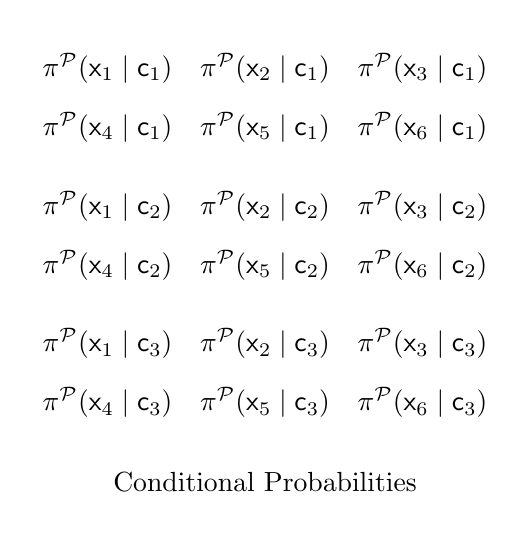
\begin{tikzpicture}[scale=1, thick]

  \foreach \c/\dy in {1/0, 2/-1.75, 3/-3.5} {
    \begin{scope}[shift={(0, \dy)}]
      \draw[white] (-3, -0.5) rectangle (3, 1.25);
      \foreach \x/\y\glyph [count=\n] in {-2/0.75, 0/0.75, 2/0.75, -2/0, 0/0, 2/0} {
        \begin{scope}[shift={(\x, \y)}]
          \node at (0, 0) { $\pi^{\mathcal{P}}(\mathsf{x}_{\n} \mid \mathsf{c}_{\c})$ };
        \end{scope}
      }
    \end{scope}
  }
  
  \begin{scope}[shift={(0, -4.5)}]
    \draw[white] (-3, -0.5) rectangle (3, 0.5);
    \node at (0, 0) { Conditional Probabilities };
  \end{scope}

\end{tikzpicture}

\end{document}  